%=====================================================================
%  Informe — Generación de animación 2D de un personaje articulado
%  mediante redes neuronales recurrentes.
%  Compilar con: pdflatex informe.tex  (dos veces)
%=====================================================================
\documentclass[10pt,twocolumn]{article}

\usepackage[utf8]{inputenc}
\usepackage[T1]{fontenc}
\usepackage[spanish]{babel}
\usepackage[margin=2cm]{geometry}
\usepackage{graphicx}
\usepackage{amsmath}
\usepackage{booktabs}
\usepackage{caption}
\usepackage{url}

\captionsetup{font=small,labelfont=bf}
\setlength{\columnsep}{0.7cm}

\title{\vspace{-1.2cm}\textbf{Generación de animación 2D de un personaje
articulado mediante redes neuronales recurrentes sobre un estado cinemático}}

\author{
  \textit{Maestría en Inteligencia Artificial --- Aprendizaje Profundo}\\
  Proyecto Final
}
\date{}

\begin{document}
\maketitle

\begin{abstract}
\noindent
Presentamos un sistema de síntesis de movimiento para un personaje 2D (un ninja
con katana) que separa de forma estricta la representación del movimiento y su
visualización. El personaje se describe mediante un \textbf{estado cinemático} de
17 variables: la posición y orientación de la cadera, sus velocidades, doce
ángulos articulares relativos y la fase del movimiento. Las coordenadas de las
articulaciones nunca se almacenan, sino que se derivan por \textbf{cinemática
directa}. Sobre esta representación construimos un conjunto de datos de
$600\times40\times17$ generado de forma procedural y entrenamos redes recurrentes
(RNN, LSTM y GRU) para predecir el siguiente estado a partir de una ventana
temporal. El mejor modelo alcanza un error cuadrático medio de validación de
$0{,}0071$ en el espacio normalizado, con errores de $\mathrm{MAE}=1{,}42$ y
$\mathrm{RMSE}=2{,}18$ en unidades físicas, y genera animaciones autoregresivas
visualmente correctas para los diez movimientos considerados. Una extensión
condicionada por acción permite además encadenar coreografías a demanda. Puesto
que la salida de la red reutiliza el mismo motor de cinemática y de render de la
etapa procedural, convertir esa salida en imagen no exigió modificar el motor
gráfico.
\end{abstract}

%=====================================================================
\section{Introducción}
%=====================================================================
La síntesis automática de movimiento es un problema central en gráficos por
computadora y videojuegos. El enfoque clásico, animar a mano fotograma a
fotograma o capturar movimiento real, resulta costoso y poco flexible. Los
métodos basados en aprendizaje profundo prometen generar movimiento continuo,
variado y controlable a partir de datos.

Una decisión determinante es \emph{qué} debe predecir la red. Si el modelo estima
directamente las coordenadas $(x,y)$ de cada articulación, nada garantiza que los
huesos conserven su longitud: pequeños errores producen extremidades que se
estiran o se encogen, un artefacto visualmente inaceptable. Por ese motivo
adoptamos una representación angular y jerárquica, en la que la red predice
ángulos relativos entre articulaciones y la geometría se reconstruye después por
cinemática directa. Así, la invariancia de las longitudes óseas deja de ser algo
que el modelo debe aprender y pasa a estar garantizado por construcción.

Las contribuciones de este trabajo son cuatro: un motor de animación esquelética
2D con cinemática directa, límites articulares y renderizado por piezas; un
generador procedural de diez movimientos que actúa como fuente de datos
etiquetados y reproducibles; el diseño y la evaluación comparada de modelos
recurrentes sobre el estado cinemático; y una variante condicionada por acción
capaz de encadenar varios movimientos consecutivos.

%=====================================================================
\section{Trabajos relacionados}
%=====================================================================
El modelado de secuencias con redes recurrentes se apoya en las celdas con
compuertas: la LSTM \cite{lstm} y, posteriormente, la GRU \cite{gru}, que logra un
desempeño comparable con menos parámetros. Ambas constituyen las arquitecturas
que comparamos en este trabajo.

En el dominio específico del movimiento, Martinez \emph{et al.} \cite{martinez}
estudiaron la predicción de movimiento humano con redes recurrentes y mostraron
que las arquitecturas simples con conexiones residuales son sorprendentemente
competitivas. Su aportación más relevante para nosotros es el diagnóstico de la
\emph{deriva} de estos modelos en horizontes largos, un fenómeno que observamos y
discutimos en la Sección~6.

Dos trabajos justifican decisiones concretas de nuestro diseño. Las
\emph{Phase-Functioned Neural Networks} de Holden \emph{et al.} \cite{pfnn}
demostraron que una variable de \textbf{fase}, que indica en qué punto del ciclo
se encuentra la acción, es determinante para lograr locomoción estable; de ahí
que incluyamos la fase dentro del propio estado. Por su parte, Villegas
\emph{et al.} \cite{nkn} incorporaron una capa de cinemática directa dentro de la
red para garantizar huesos de longitud constante, idea que nosotros aplicamos
situando la cinemática directa fuera del modelo, como paso de decodificación.

Nuestro escenario se diferencia de todos ellos en que es bidimensional y
controlado: el generador procedural provee datos ilimitados, perfectamente
etiquetados y sin ruido de captura, lo que permite estudiar el efecto de la
arquitectura sin confundirlo con las limitaciones de los datos.

%=====================================================================
\section{Representación cinemática y renderizado}
%=====================================================================
\subsection{Esqueleto y cinemática directa}
El personaje es un árbol jerárquico de 17 nodos cuya raíz es la cadera. De la
cadera nacen el tronco, y de éste el cuello, la cabeza y ambos brazos, así como
las dos piernas; la katana cuelga de la mano derecha mediante una articulación
adicional. Cada hueso posee una longitud constante $\ell_j$, un ángulo de reposo
$\beta_j$ relativo a su padre y, cuando es articulado, una variable
$\theta_j$. La posición de cada nodo se obtiene de forma recursiva:
\begin{align}
\phi_j &= \phi_{\text{padre}(j)} + \beta_j + s_j\,\theta_j, \\
\mathbf{p}_j &= \mathbf{p}_{\text{padre}(j)} + \ell_j\,(\cos\phi_j,\ \sin\phi_j),
\end{align}
donde $\phi_j$ es el ángulo absoluto del hueso y $s_j\in\{-1,+1\}$ codifica el
sentido anatómico de la flexión, pues el codo flexiona hacia delante y la rodilla
hacia atrás. La raíz parte de $(\text{root\_x},\text{root\_y})$ con orientación
$\text{root\_rotation}+90^\circ$.

Cada articulación tiene además \textbf{límites físicos} que se aplican por
saturación antes de propagar la cadena: codo $[0^\circ,150^\circ]$, rodilla
$[0^\circ,140^\circ]$, cuello $[-40^\circ,40^\circ]$ y espalda
$[-30^\circ,30^\circ]$. Esto impide poses anatómicamente imposibles incluso si el
modelo predice valores fuera de rango y, como veremos, estabiliza la generación.

\subsection{Del estado al personaje: el proceso de render}
La motivación del renderizado es cerrar el ciclo de validación: un vector de
números sólo resulta útil si podemos \emph{ver} si el movimiento es correcto. El
error cuantitativo no distingue entre una desviación irrelevante y otra que
arruina la pose; la inspección visual sí lo hace.

El proceso consta de cuatro pasos, idénticos tanto para el generador procedural
como para la red (Fig.~\ref{fig:pipeline}). En primer lugar, se recorre el árbol
aplicando las ecuaciones (1) y (2), con lo que se obtienen el ángulo absoluto y
la posición de los 17 nodos. En segundo lugar, a cada hueso le corresponde una
imagen PNG con fondo transparente, generada también de forma procedural: torso,
cabeza, cuello, brazo, antebrazo, mano, muslo, pantorrilla, pie y katana. En
tercer lugar, cada pieza se dibuja apuntando hacia la derecha con su pivote
situado en el borde izquierdo, se rota exactamente $\phi_j$ grados alrededor de
ese pivote y se coloca sobre la articulación padre; como el pivote coincide
siempre con la articulación, las piezas nunca se separan entre sí. Finalmente,
las piezas se componen de atrás hacia delante y se convierten a coordenadas de
pantalla. La cámara sigue a la cadera en horizontal, para que las traslaciones no
saquen al personaje del encuadre, pero no en vertical, de modo que los saltos
siguen siendo visibles.

La consecuencia de diseño más importante es que el motor de render desconoce si
el estado procede de una fórmula matemática o de una red neuronal, por lo que
sustituir el generador por el modelo entrenado no obligó a modificarlo.

\begin{figure}[t]
  \centering
  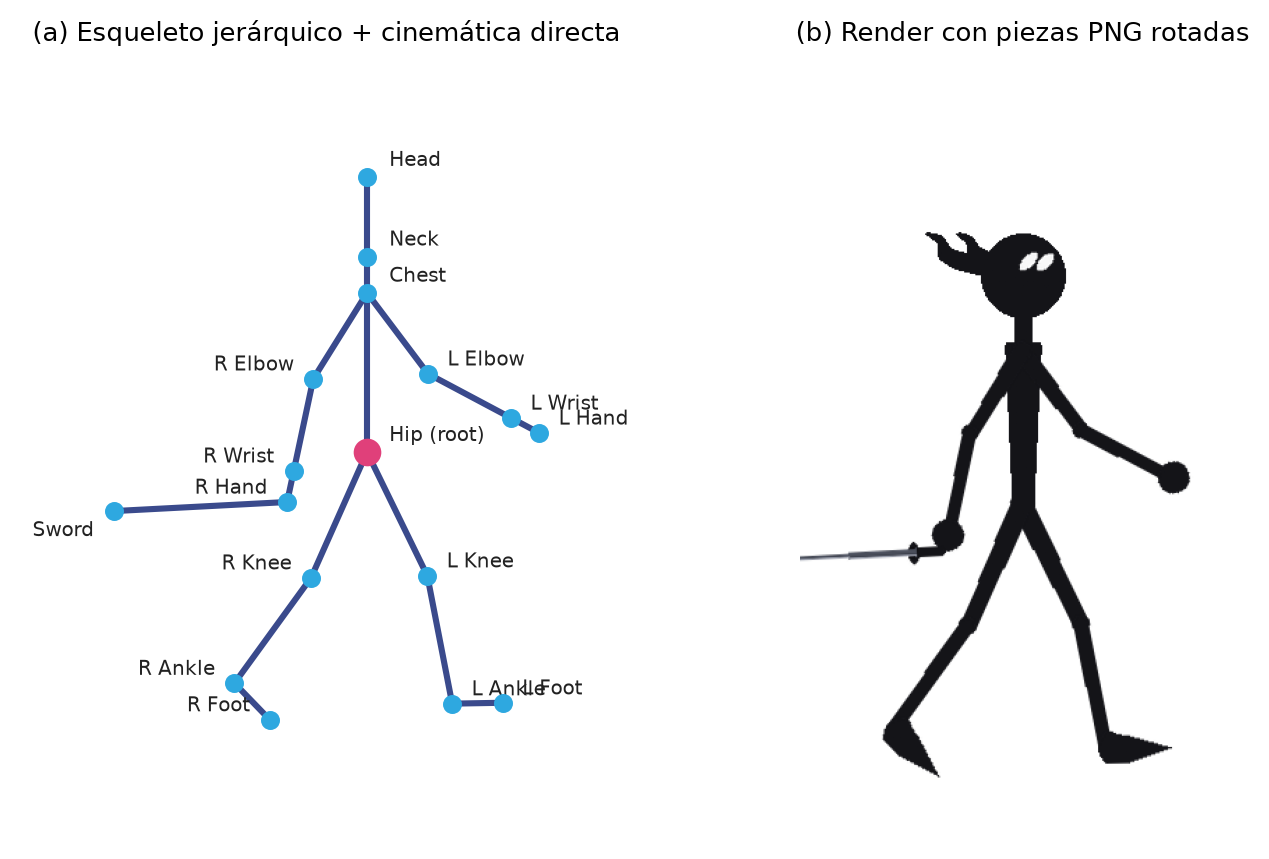
\includegraphics[width=\linewidth]{figs/fig_pipeline.png}
  \caption{(a) Árbol jerárquico y coordenadas obtenidas por cinemática directa.
  (b) Render final componiendo las piezas PNG rotadas sobre sus pivotes.}
  \label{fig:pipeline}
\end{figure}

%=====================================================================
\section{Construcción del conjunto de datos}
%=====================================================================
\subsection{Cómo se generan las secuencias}
Los datos no proceden de captura de movimiento sino de un \textbf{generador
procedural} propio. Para cada movimiento definimos los ángulos articulares como
funciones continuas del tiempo normalizado $t\in[0,1)$, construidas con senos,
cosenos, interpolaciones suaves y curvas de campana. La continuidad de estas
funciones es precisamente lo que hace que la animación resultante se perciba
fluida al reproducirse a 30 fotogramas por segundo.

Conviene verlo en un caso concreto. La patada se modela con una curva de campana
centrada en el instante del impacto,
\begin{equation}
e(t)=\exp\!\left(-\frac{(t-t_{g})^{2}}{2\sigma^{2}}\right),
\end{equation}
que vale cero al principio y al final y alcanza su máximo en el golpe. Los
ángulos de la pierna derecha se obtienen interpolando entre la postura de reposo
y la de impacto mediante ese factor:
\begin{align}
\text{right\_hip}(t)  &= \mathrm{lerp}(-10^\circ,\ r,\ e(t)),\\
\text{right\_knee}(t) &= \mathrm{lerp}(70^\circ,\ 8^\circ,\ e(t)).
\end{align}
Es decir, la cadera eleva la pierna al frente mientras la rodilla se extiende, y
ambas regresan después a la posición inicial. La Tabla~\ref{tab:patada} muestra
los valores reales producidos por el generador para una patada de 30 fotogramas:
en el fotograma~15 la cadera alcanza $97{,}2^\circ$ y la rodilla se estira hasta
$10{,}1^\circ$, que es el instante del impacto.

\begin{table}[t]
\centering
\footnotesize
\caption{Valores generados para una patada real (30 fotogramas). Cada fila es una
pose completa; se muestran cuatro de las diecisiete variables.}
\label{tab:patada}
\begin{tabular}{@{}rrrrr@{}}
\toprule
Fotograma & right\_hip & right\_knee & torso\_angle & root\_y \\
\midrule
0  & $-9{,}5$ & $69{,}7$ & $0{,}0$ & $240{,}0$ \\
6  & $9{,}4$  & $59{,}2$ & $1{,}7$ & $241{,}4$ \\
12 & $90{,}5$ & $13{,}9$ & $9{,}1$ & $247{,}2$ \\
15 & $\mathbf{97{,}2}$ & $\mathbf{10{,}1}$ & $9{,}7$ & $247{,}7$ \\
18 & $59{,}1$ & $31{,}4$ & $6{,}2$ & $245{,}0$ \\
24 & $-3{,}7$ & $66{,}5$ & $0{,}6$ & $240{,}5$ \\
\bottomrule
\end{tabular}
\end{table}

Un aspecto esencial es que los parámetros de estas funciones se \textbf{sortean
al azar en cada ejecución}. En la patada varían el instante del golpe
$t_g\sim U(0{,}45,\,0{,}60)$, la velocidad del ataque (que controla el ancho
$\sigma$ de la campana) y el alcance $r\sim U(85^\circ,105^\circ)$; en la marcha
varían la longitud del paso, la amplitud de los brazos y la inclinación del
torso, y en el salto, su altura. Gracias a ello nunca se generan dos secuencias
idénticas, lo que impide que la red memorice trayectorias y actúa como una forma
intensiva de aumento de datos.

\subsection{Estructura del tensor}
Generamos 60 variantes de cada uno de los 10 movimientos, fijando la duración en
40 fotogramas para obtener un tensor rectangular. El resultado tiene forma
$(N,T,D)=(600,\,40,\,17)$, y conviene interpretar cada eje por separado.

El primer eje recorre las \textbf{600 secuencias}, cada una de las cuales es una
ejecución completa de una acción. Están ordenadas por movimiento, de modo que las
secuencias $0$ a $59$ son variantes de \emph{idle}, las $60$ a $119$ de
\emph{walk}, y así sucesivamente. El segundo eje recorre los \textbf{40
fotogramas} de esa ejecución: cada posición es un instante de tiempo. El tercer
eje recorre las \textbf{17 variables} del estado, descritas en la
Tabla~\ref{tab:estado}.

Un ejemplo concreto aclara la lectura. La secuencia $430$ pertenece al grupo de
las patadas, que ocupa los índices $420$ a $479$. El elemento
\texttt{data[430,\,22,\,13]} contiene el ángulo de la cadera derecha
(variable~13) en el fotograma~22 de esa ejecución, y su valor real es
$103{,}9^\circ$, que corresponde al instante de máxima elevación de la pierna.
En ese mismo fotograma, \texttt{data[430,\,22,\,14]} vale $8{,}3^\circ$, es
decir, la rodilla está prácticamente extendida: exactamente la mecánica del
impacto descrita más arriba.

Las rebanadas del tensor tienen una interpretación igualmente clara.
\texttt{data[430,\,22,\,:]} es un vector de 17 números que constituye la
\emph{pose completa} del personaje en ese instante, la fotografía instantánea de
todo el cuerpo. En cambio, \texttt{data[430,\,:,\,13]} es la \emph{trayectoria
temporal} de esa única articulación a lo largo de toda la patada, es decir, la
curva ascendente y descendente que ilustra la Tabla~\ref{tab:patada}.

Merece subrayarse que una fila no contiene un ángulo aislado, sino los doce
ángulos articulares de forma simultánea junto con la raíz, sus velocidades y la
fase. Una acción es, por tanto, una trayectoria suave de poses en
$\mathbb{R}^{17}$.

\begin{table}[t]
\centering
\scriptsize
\caption{Significado de las $D=17$ columnas del vector de estado.}
\label{tab:estado}
\begin{tabular}{@{}clll@{}}
\toprule
\# & Variable & Unidad & Significado \\
\midrule
0  & \texttt{root\_x}         & px & traslación horizontal de la cadera \\
1  & \texttt{root\_y}         & px & altura de la cadera (saltos) \\
2  & \texttt{root\_rotation}  & $^\circ$ & orientación global del cuerpo \\
3  & \texttt{velocity\_x}     & px/f & velocidad horizontal de la raíz \\
4  & \texttt{velocity\_y}     & px/f & velocidad vertical de la raíz \\
5  & \texttt{torso\_angle}    & $^\circ$ & flexión de la espalda $[-30,30]$ \\
6  & \texttt{neck\_angle}     & $^\circ$ & cuello $[-40,40]$ \\
7  & \texttt{left\_shoulder}  & $^\circ$ & hombro izq. $[-170,170]$ \\
8  & \texttt{left\_elbow}     & $^\circ$ & codo izq. $[0,150]$ \\
9  & \texttt{right\_shoulder} & $^\circ$ & hombro der. $[-170,170]$ \\
10 & \texttt{right\_elbow}    & $^\circ$ & codo der. $[0,150]$ \\
11 & \texttt{left\_hip}       & $^\circ$ & cadera izq. $[-120,120]$ \\
12 & \texttt{left\_knee}      & $^\circ$ & rodilla izq. $[0,140]$ \\
13 & \texttt{right\_hip}      & $^\circ$ & cadera der. $[-120,120]$ \\
14 & \texttt{right\_knee}     & $^\circ$ & rodilla der. $[0,140]$ \\
15 & \texttt{sword\_angle}    & $^\circ$ & katana respecto de la mano \\
16 & \texttt{phase}           & --- & progreso normalizado $[0,1)$ \\
\bottomrule
\end{tabular}
\end{table}

La inclusión de las velocidades y de la fase no es accesoria. Las velocidades,
calculadas como diferencias finitas de la raíz, aportan información dinámica de
primer orden que de otro modo la red tendría que inferir. La fase, inspirada en
\cite{pfnn}, indica en qué punto del ciclo se encuentra la acción y ayuda a
desambiguar poses visualmente parecidas pero temporalmente opuestas, como la
pierna subiendo frente a la pierna bajando.

\subsection{Ventanas temporales y normalización}
Convertimos las secuencias en pares supervisados mediante una \textbf{ventana
deslizante}: las poses de las posiciones $i$ a $i+W-1$ se usan para predecir la
pose $i+W$, con $W=16$. La partición entre entrenamiento y validación se realiza
\textbf{por secuencias} y no por ventanas, en proporción $85/15$, para evitar que
fragmentos de una misma ejecución aparezcan en ambos conjuntos. Se obtienen así
$12\,240$ ventanas de entrenamiento, con
$X\in\mathbb{R}^{12240\times16\times17}$, y $2\,160$ de validación.

Como las variables tienen escalas muy dispares, pues conviven píxeles y grados,
se estandarizan mediante $\tilde{x}=(x-\mu)/\sigma$ con estadísticos calculados
únicamente sobre el conjunto de entrenamiento. El normalizador se guarda en
disco porque resulta imprescindible durante la inferencia: la red opera en el
espacio normalizado y su salida debe deshacerse esa transformación antes de
renderizar.

%=====================================================================
\section{Arquitectura del modelo}
%=====================================================================
El problema se formula como una regresión autoregresiva: dada la ventana
$\mathbf{X}=(\tilde{\mathbf{s}}_{i},\dots,\tilde{\mathbf{s}}_{i+W-1})$, se debe
predecir $\tilde{\mathbf{s}}_{i+W}$. La red consta de cuatro elementos
encadenados. Primero, una pila de dos capas recurrentes con 64 unidades ocultas y
\emph{dropout} de $0{,}1$ entre ellas, que procesa los 16 fotogramas de la
ventana. Segundo, una extracción del vector correspondiente al \textbf{último
paso temporal} de la salida recurrente, que resume el contexto de toda la
ventana. Tercero, una capa densa de 64 unidades con activación ReLU. Y cuarto,
una capa densa final de 17 salidas, una por cada variable del estado.

El tipo de celda recurrente es un único parámetro configurable, lo que permite
comparar RNN simple, LSTM y GRU manteniendo idéntico el resto del sistema. En su
versión GRU el modelo tiene $46\,161$ parámetros entrenables, una cifra modesta
que confirma que la dificultad del problema reside en la representación y no en
la capacidad del modelo.

El entrenamiento minimiza el error cuadrático medio sobre el espacio normalizado,
donde todas las variables pesan por igual, mediante el optimizador Adam con tasa
de aprendizaje $10^{-3}$, lotes de 256 muestras y 15 épocas, conservando los
pesos que producen la menor pérdida de validación.

\paragraph{Variante condicionada por acción.}
El modelo anterior continúa el movimiento que observa, pero no permite
\emph{solicitar} una acción concreta. Para encadenar coreografías añadimos a la
entrada de cada paso temporal un vector \emph{one-hot} que indica la acción
deseada, de manera que la dimensión de entrada pasa de 17 a $17+10=27$. Este
modelo se entrena sobre secuencias compuestas, esto es, concatenaciones de dos o
tres movimientos con transiciones interpoladas, para que aprenda también los
tránsitos entre acciones. Se emplearon $12\,108$ ventanas y una GRU de 96
unidades durante 16 épocas, alcanzando una pérdida final de $0{,}0162$.

%=====================================================================
\section{Resultados y discusión}
%=====================================================================
\subsection{Convergencia y error}
La Fig.~\ref{fig:loss} muestra las curvas de pérdida del modelo GRU. El error de
validación desciende de $0{,}3187$ a $0{,}0071$ a lo largo de 15 épocas de forma
monótona y sin separarse de la curva de entrenamiento, lo que indica ausencia de
sobreajuste. Este comportamiento era previsible, ya que el generador provee
variabilidad ilimitada y opera como una forma intensiva de aumento de datos.

Sobre las $2\,160$ ventanas de validación, el error de predicción a un paso
expresado en unidades físicas es de $\mathrm{MAE}=1{,}42$ y
$\mathrm{RMSE}=2{,}18$. Dado que los ángulos recorren rangos de hasta
$150^\circ$, un error medio próximo a $1{,}4^\circ$ resulta visualmente
imperceptible.

\begin{figure}[t]
  \centering
  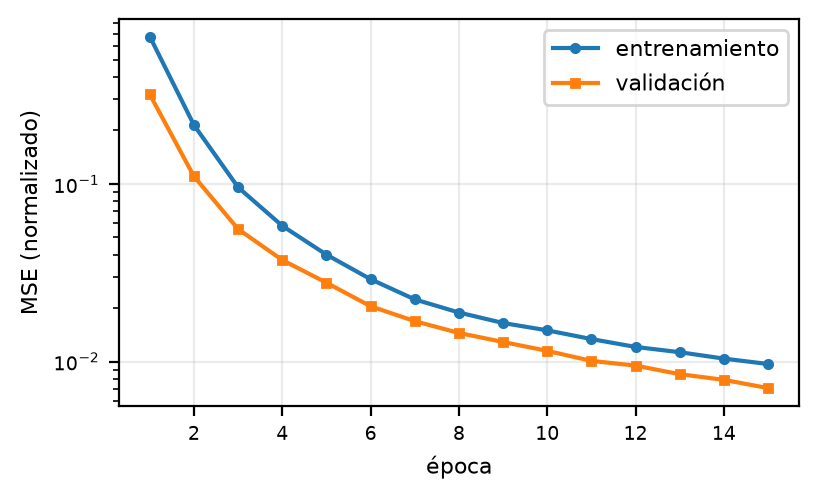
\includegraphics[width=0.92\linewidth]{figs/fig_loss.png}
  \caption{Curvas de pérdida (error cuadrático medio normalizado, escala
  logarítmica) del modelo GRU.}
  \label{fig:loss}
\end{figure}

\subsection{Comparación de arquitecturas}
La Tabla~\ref{tab:comp} compara las tres celdas en igualdad de condiciones, con
10 épocas cada una. Las celdas con compuertas superan claramente a la RNN simple
en todas las métricas de error. Entre ellas, LSTM y GRU quedan muy próximas, con
un MAE de $1{,}73$ frente a $1{,}78$, pero la GRU entrena aproximadamente un
15\,\% más rápido por disponer de menos parámetros por celda. La RNN simple es la
más veloz y a la vez la menos precisa, y cualitativamente es también la que antes
se degrada en generación larga. Este patrón coincide con lo reportado en
predicción de movimiento humano \cite{martinez}.

\begin{table}[t]
\centering
\footnotesize
\caption{Comparación de arquitecturas (10 épocas, mismo conjunto y partición).}
\label{tab:comp}
\begin{tabular}{@{}lccccc@{}}
\toprule
Modelo & $t_{\text{entren}}$ (s) & $t_{\text{infer}}$ (s) & MSE val. & MAE & RMSE \\
\midrule
RNN  & 2{,}11 & 0{,}0039 & 0{,}0137 & 1{,}929 & 3{,}577 \\
LSTM & 6{,}65 & 0{,}0075 & \textbf{0{,}0118} & \textbf{1{,}727} & \textbf{3{,}107} \\
GRU  & 5{,}64 & 0{,}0073 & 0{,}0122 & 1{,}778 & 3{,}303 \\
\bottomrule
\end{tabular}
\end{table}

\subsection{Evaluación cualitativa}
La evaluación visual constituye la prueba definitiva. Partiendo de una semilla de
16 fotogramas reales, la red genera de forma autoregresiva los 24 restantes para
los diez movimientos, y todos resultan reconocibles y anatómicamente plausibles.
La Fig.~\ref{fig:res}(a) muestra una patada generada por el modelo en la que la
cadera se eleva y la rodilla se extiende en el instante del impacto,
reproduciendo la mecánica descrita en la Tabla~\ref{tab:patada}. La
Fig.~\ref{fig:res}(b) muestra una secuencia encadenada de 124 fotogramas en la
que el personaje corre, salta y ataca de forma continua.

\begin{figure}[t]
  \centering
  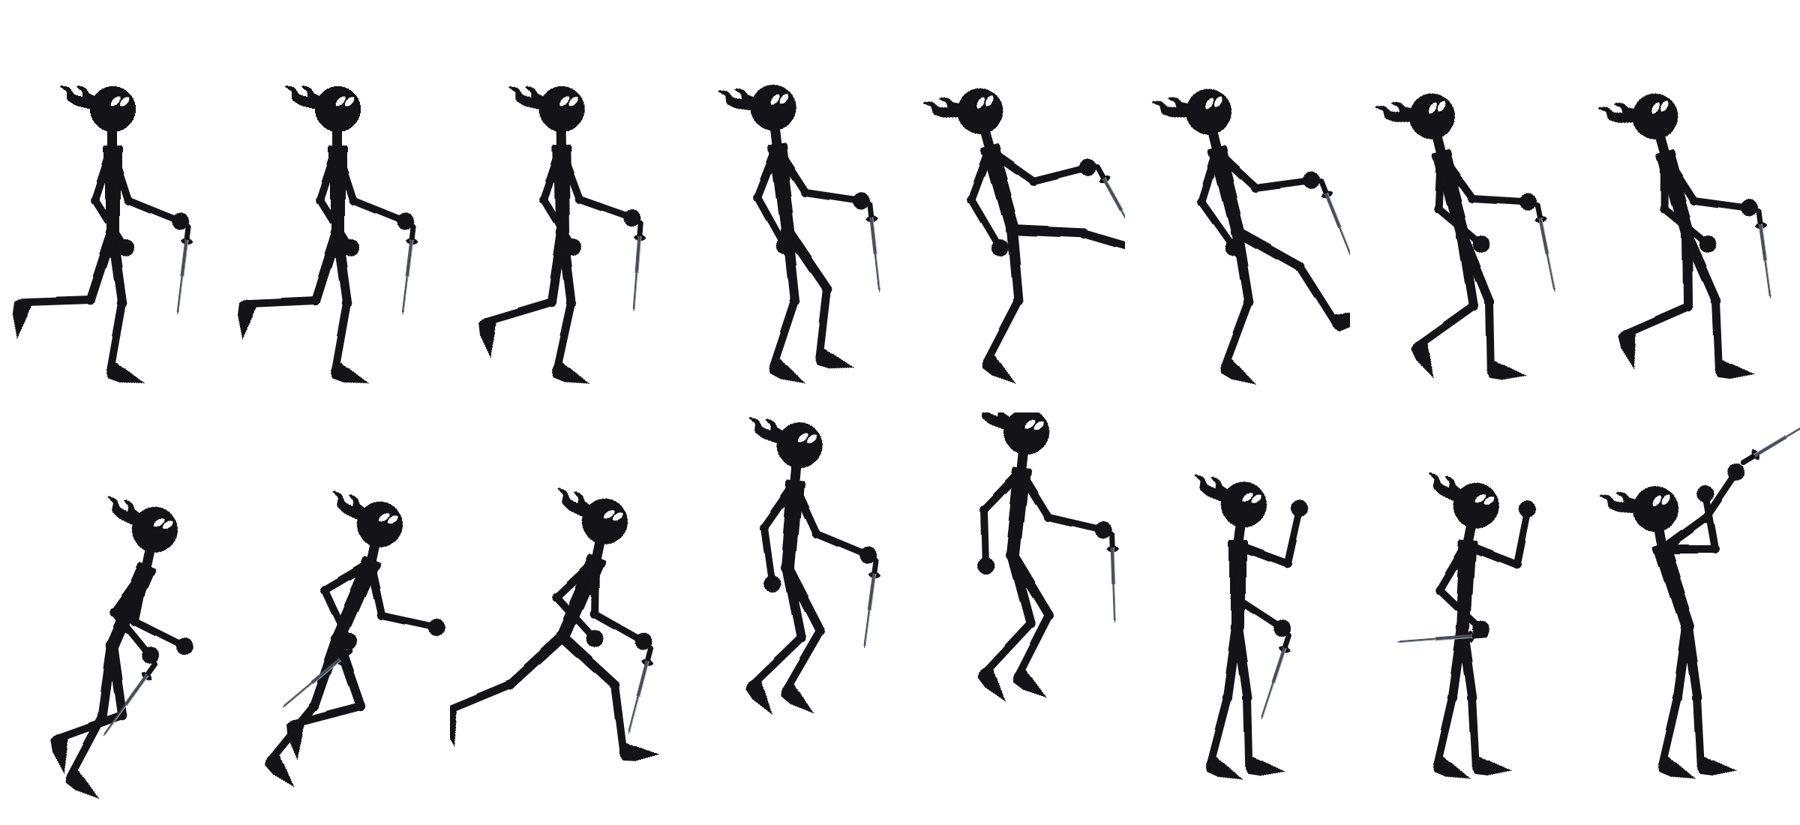
\includegraphics[width=\linewidth]{figs/fig_results.png}
  \caption{(a) Patada generada autoregresivamente por la GRU. (b) Secuencia
  encadenada en la que el ninja corre, salta y ataca, con transiciones suaves.}
  \label{fig:res}
\end{figure}

\subsection{Discusión y limitaciones}
Observamos dos fenómenos relevantes. El primero es que la saturación a los
límites articulares actúa como regularizador durante la inferencia: al reinyectar
en la ventana una predicción ya saturada, se evita que pequeños errores se
acumulen hasta producir poses imposibles. El segundo es que la estabilidad
depende de la acción. Los movimientos en contacto con el suelo, como correr,
patear o cortar, se sostienen bien, mientras que el salto, que incluye una fase
aérea donde la raíz sigue una parábola, tiende a degradarse en horizontes largos.
Este comportamiento es consistente con la deriva descrita por Martinez
\emph{et al.} \cite{martinez} y constituye la principal limitación del sistema.
Su origen está en el desajuste entre el entrenamiento, que emplea siempre valores
reales como entrada, y la inferencia, que realimenta las propias predicciones del
modelo; el \emph{scheduled sampling} \cite{scheduled} es el remedio estándar para
este problema.

%=====================================================================
\section{Salidas del modelo: interpretación y ejecución}
%=====================================================================
\paragraph{Qué devuelve la red.} Una sola invocación produce un vector de 17
números normalizados correspondientes al \textbf{siguiente} fotograma. No se
trata de una imagen ni de una clase, sino de una pose. Para interpretarlo se
deshace la normalización mediante $x=\tilde{x}\sigma+\mu$ y se lee cada
componente según la Tabla~\ref{tab:estado}; por ejemplo, un valor de
\texttt{right\_knee} cercano a $10^\circ$ indica una pierna casi extendida, y un
\texttt{root\_y} elevado señala que el personaje se encuentra en el aire.

\paragraph{Cómo se obtiene una animación completa.} Repitiendo el paso anterior
de forma autoregresiva. Se parte de una ventana semilla, se predice la pose
siguiente, se añade al final de la ventana y se descarta la más antigua. Cada
pose se convierte en un diccionario de estado, se satura a los límites
articulares, se transforma en coordenadas mediante cinemática directa y se
dibuja.

\paragraph{Ejecución.} El proyecto está organizado en módulos independientes y el
visualizador interactivo se lanza con \texttt{python main.py}. El cuaderno
\texttt{development.ipynb} contiene, en secciones ejecutables de forma
independiente, la validación del esqueleto y la cinemática, el entrenamiento, el
encadenado de acciones y un reproductor de las secuencias predichas. Los
artefactos \texttt{best\_model.pt}, \texttt{cond\_model.pt} y
\texttt{normalizer.npz} permiten reproducir la inferencia sin reentrenar. La
implementación emplea PyTorch.

%=====================================================================
\section{Conclusiones}
%=====================================================================
Hemos mostrado que una red recurrente compacta, de unos 46 mil parámetros, es
capaz de aprender y regenerar diez movimientos acrobáticos de un personaje
articulado cuando el problema se plantea sobre un estado cinemático angular en
lugar de sobre coordenadas. La cinemática directa garantiza por construcción que
las longitudes de los huesos se conserven, y los límites articulares aportan una
regularización física que estabiliza la generación autoregresiva.

Las celdas con compuertas superan con claridad a la RNN simple y resultan
equivalentes entre sí, con ventaja de coste computacional para la GRU.
Cualitativamente, las diez acciones son reconocibles y el condicionamiento por
acción permite encadenar coreografías a demanda.

Las limitaciones principales son la degradación del salto en horizontes largos,
la predicción de la posición absoluta de la raíz, que acumula error, y el carácter
sintético de los datos, por lo que la generalización a captura real queda sin
verificar. Como trabajo futuro proponemos entrenar con \emph{scheduled sampling}
\cite{scheduled}, predecir incrementos del estado en lugar de valores absolutos
reconstruyendo la raíz por integración de la velocidad, modular los pesos con la
fase siguiendo a \cite{pfnn}, y validar el procedimiento sobre datos reales de
captura de movimiento.

%=====================================================================
\begin{thebibliography}{9}\footnotesize
\bibitem{lstm} S.~Hochreiter and J.~Schmidhuber, ``Long Short-Term Memory,''
\emph{Neural Computation}, vol.~9, no.~8, pp.~1735--1780, 1997.

\bibitem{gru} K.~Cho, B.~van Merriënboer, C.~Gulcehre, D.~Bahdanau, F.~Bougares,
H.~Schwenk, and Y.~Bengio, ``Learning Phrase Representations using RNN
Encoder--Decoder for Statistical Machine Translation,'' in \emph{EMNLP}, 2014.

\bibitem{martinez} J.~Martinez, M.~J.~Black, and J.~Romero, ``On Human Motion
Prediction Using Recurrent Neural Networks,'' in \emph{CVPR}, 2017.

\bibitem{pfnn} D.~Holden, T.~Komura, and J.~Saito, ``Phase-Functioned Neural
Networks for Character Control,'' \emph{ACM Trans. Graph. (SIGGRAPH)}, vol.~36,
no.~4, 2017.

\bibitem{nkn} R.~Villegas, J.~Yang, D.~Ceylan, and H.~Lee, ``Neural Kinematic
Networks for Unsupervised Motion Retargetting,'' in \emph{CVPR}, 2018.

\bibitem{scheduled} S.~Bengio, O.~Vinyals, N.~Jaitly, and N.~Shazeer,
``Scheduled Sampling for Sequence Prediction with Recurrent Neural Networks,'' in
\emph{NeurIPS}, 2015.
\end{thebibliography}

\end{document}
